\documentclass[a4paper,12pt]{article}
\usepackage{hyperref}
\usepackage{times}
\usepackage{comment}
\usepackage{titlesec}
\usepackage[pdftex]{graphicx}

\usepackage{geometry}
\geometry{lmargin=1.5cm,rmargin=1.5cm,height=25cm}
\renewcommand{\thesubsection}{\Roman{subsection}}

\begin{document}

\title{THE ICON OF ST. PAUL\\ at the Wignacourt Museum, Rabat, Malta}
\author{Joanna Lace} 
\date{}%May 2009}
\maketitle 

\begin{figure}[htbp]
\centering
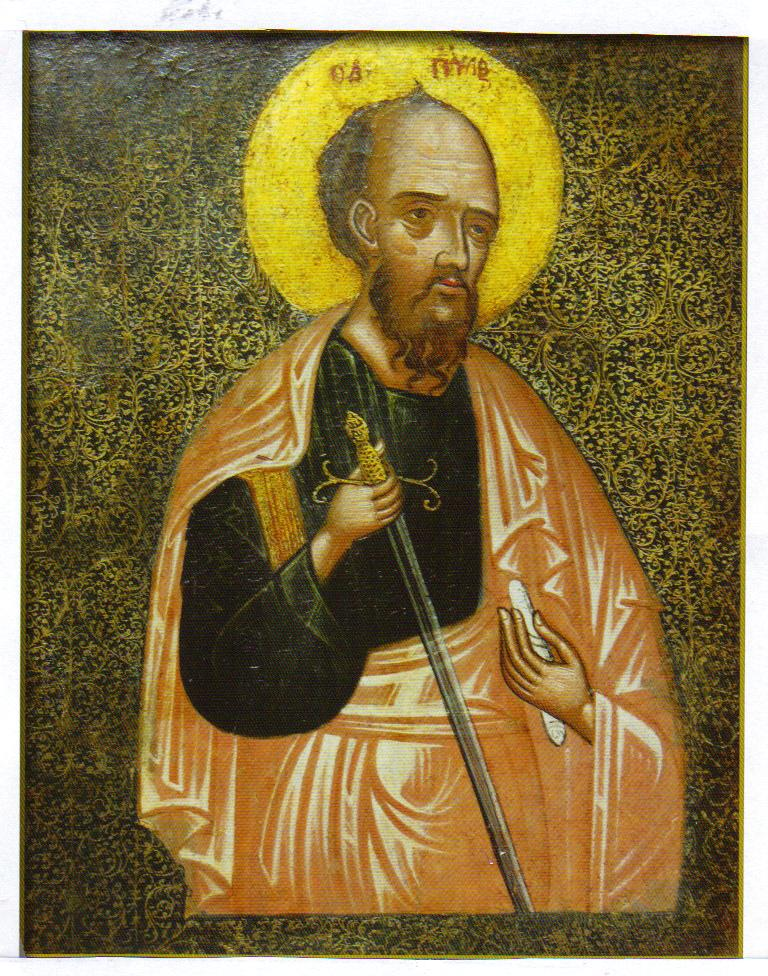
\includegraphics[width=12cm]{IconStPaul.png}
\caption 
{\it } 
\end{figure}
This image of St.~Paul is an icon, and one that is particularly
interesting for the way the artist has inserted western iconography in
an image otherwise mainly constructed along the lines of eastern
Christian art.  In both traditions the receding hair and long nose
have remained instantly recognisable since their description in the
second century Acts of Paul, and the attribute he carries---a book or
a rotolo symbolising his famous epistles---is also common to both.

An icon may be seen as `art', and subject to artistic judgment, but
for the eastern orthodox Christian, it is a visual aid to his
devotion, an interactive medium between his every-day world and the
eternal and universal world of Christ, and the artist's aim is to
inspire this devotion.  Following the eastern tradition, this artist
has identified for the worshipper St.~Paul's physical persona by
following the established iconographic canon, whereby different
classes of saints---apostles, bishops, soldiers and others---are first
identified by their clothing, and then further identified by the
colour and arrangement of hair and beard.  Our figure duly wears the
antique tunic and \textit{himation} (cloak) of an apostle, with the hair and
beard of St.~Paul.  However, it is the style in which these
iconographic features are presented that is all-important for the
eastern artist, expressing as it does the essence of a personality,
providing the essential key to our understanding of St.~Paul's
spiritual role.  And the means employed are symbolic rather than
naturalistic.  A useful study of such symbolism explains some of the
stylistic features this artist includes.  [H.~Maguire, \textit{The
    Icons of their Bodies: Saints and their Images in Byzantium},
  Princeton 1996]

Firstly, as regards the physical form of a saint, form follows
function, varying according to his life's role: corporality and
movement increase according to his closeness to Christ's life on
earth.  The bodies of aesthetics, monks, and clergy, for instance are
shown with a deliberate lack of emphasis, often with a lack of
modelling, whereas St.~Paul, whose earthly life followed closely that
of Christ, and who was a brave and indefatigable traveller, is seen
here wearing drapery that appears inflated, giving his figure a solid,
well-rounded outline.  His spirituality is suggested by a clear-cut
outline to the entire figure, the absence of any reference to a
natural environment (horizon, landscape, etc.), a background
completely closed off by decorative patterning: all these emphasise
the saint’s existence in a timeless world beyond our own.  Within
this timeless world the modelling of his cloak symbolises his earthly
activity: it is schematic, pronounced and energetic.  It is also
interesting that the particular geometric form of this style of
modelling, with its long parallel lines, was originally an optical
device used by eastern-trained artists when creating large figures in
mosaic high up in the domes of churches, where traditional modelling
using tiny tesserae was unintelligible from far below.  These figures
were always the most sacred, most often those of Christ and the
Virgin.  Over time this design took on an iconographical meaning
associated with the holiest images in other contexts, a mark of
sanctity, used even on small icons. [See O.~Demus, \textit{Byzantine Mosaic
  Decoration}, 1976, pp.~38-9.]

Our first glance however, will be drawn, by soft high-lighting, to the
sources of St.~Paul's particular gift to all Christians: his head, as
the seat of his unique intelligence, and his hands, in one of which he
holds the attribute which identifies for the worshipper the category
of saint to which he belongs: the epistles he wrote, and which are for
Christians an everlasting inspiration.  The importance of category in
identifying a saint is incidentally born out in the case of St~Thekla.
Female saints usually carry a simple cross, but in her case, as a
close disciple of St.~Paul, she carries a book.

In St.~Paul's other hand he holds a sword, an attribute that only in
western iconography denotes the manner of his martyrdom – in Paul's
case beheading by the sword.  In eastern icons attributes are more
important for establishing the category of saint to which an
individual belonged.  A sword, for example, is the attribute of a
warrior saint.

In conclusion it should be said that this western element, together
with a certain 'western' smoothing out of the classic facial lines of
a saint as composed in eastern Christian terms, in no way detract from
the appeal of the icon.  This St.~Paul is not monumental; his focus is
inward, and quite in keeping with the qualities evoked by the artist's
interpretation of his major role.

\subsection*{APPENDIX} % --- ICON OF ST. PAUL}

Features traced to countries under orthodox influence:

\begin{enumerate}
\item BACKGROUND DESIGN: The same pattern was used for the background
  to the four paintings on the wings of a triptych in the collection
  of the Holy Monastery of St.~Catherine, Sinai, Egypt.  The paintings
  are now considered to be by a French artist working in the Levant,
  and are dated to the mid-thirteenth century. [See R.~Cormack,
    \textit{Icons}, British Museum Press 2007, p.~79, Fig.~50; and R.~Cormack
    and M.~Vassilaki, \textit{Byzantium}, 330--1453, Royal Academy London
    2008--09, p.~363, Fig.~53.]

This background imitates the metal covering or riza sometimes given to
Byzantine icons, and those from orthodox areas after 1453, from Cyprus
and the Balkans; and later very popular in Russia.

\item BEARD OF ST.~PAUL: Its unruly curls are seen in the work of
  artists working each side of the Adriatic coast during the
  fourteenth century.  See S.~Papetti, \textit{L'Aquila e il Leone: L'Arte
  Veneta a Fermo, Sant'Epidio a Mare e nel Fermano}, Catalogue of
  exhibition held March-September 2006, p.~108.

\item PARTICULAR FORM OF THE SCROLL OR ROTOLO: small, slim,
  'cigar-shaped': Seen in work by the Maestro d/Elsino, formerly known
  as the Ceruda Master, active at the end of the fourteenth century.
  See ed. F.~Flores d'Arcais, \textit{Il Trecento adriatico}, catalogue of
  exhibition held in Castel Sismondo, Rimini, August-December 2002,
  p.~216, Pl.~58; also \textit{L'Aquila e il Leone}, op.cit. above, p.~101,
  Pl.~6.

\item 
RECTILINEAR HIGHLIGHTS, ROUNDED HAND holding sword, OUTLINES IN BLACK:
Seen in St~Clement, Ohrid, Macedonia. See P.~Muller, Famous Icons –
12th to 18th Centuries, Belgrade 1984, Pl.~34 The Apostle Matthew, 15th
century.

\end{enumerate}


\subsection*{AFTERWORD}

\underline{The Sword of St. Paul}: Fine details of the pommel of the
sword have been revealed by the recent cleaning of the icon: these
require further study.

\bigskip
\noindent
\copyright\ Joanna Lace, May 2009.
\end{document}

ed. John Azzopardi, \textit{Salve Pater Paule: a collection of Essays and
Exhibition Catalogue of Pauline Art}, Rabat, Malta, 2009, pp. 99-100.
